\section{РУКОВОДСТВО ПОЛЬЗОВАТЕЛЯ}
Приложение сбора статистики и анализа данных в тексте предоставялет возможность для:
\begin{itemize}
\item собирать информацию о фильмах из интернет ресурсов;
\item собирать информацию о товарах из интернет магазнов;
\item обучать модели Child-Sum Tree LSTM\@;
\item производить анализ тональностей предложений.
\end{itemize}

\subsection{Требование к аппаратному и программному обеспечению}
Минимальные требования для работы системы:
\begin{itemize}
\item процессор Intel Сore i3;
\item 4 гигабайта оперативной памяти;
\item операционная система семейства Unix.
\end{itemize}

Для работы визуализации необходимо наличие браузера с поддержкой Javascript на компьютере пользователя. Поддерживаются следующие типы браузеров:
\begin{itemize}
\item Safari;
\item Google Chrome;
\item Mozilla Firefox;
\item Opera 15;
\item Internet Explorer 9+.
\end{itemize}

\subsection{Руководство по установке системы}
Для работы системы необходимо установить множество пакетов Python. Чтобы не нарушить системные зависимости рекомендуется установить приложение pipenv, которое позволит создать среду отдельно от системной:
\medskip
\begin{lstlisting}[style=Python]
  sudo pip3 install pipenv
\end{lstlisting}
\medskip

После этого в папке с проектом можно создать локальную среду Python. В первый раз эта команда создаст необходимую минимальную среду для работы с локальным python, в последующие запуски она будет использовать ранее созданую среду:
\medskip
\begin{lstlisting}[style=Python]
  pipenv shell
\end{lstlisting}
\medskip

Установку пакетов лучше производить также через pipenv с помощью следующей команды:
\medskip
\begin{lstlisting}[style=Python]
  pipenv install <имя пакета>
\end{lstlisting}
\medskip

В случае же, если пользователь решил пользоваться стандартными средствами, то установку пакетов можно проивести и с помощью  pip:
\medskip
\begin{lstlisting}[style=Python]
  sudo pip install <имя пакета>
\end{lstlisting}
\medskip

Необходимо установить следующие пакеты в перечисленном порядке:
\begin{itemize}
\item six;
\item backcall;
\item decorator;
\item parso версии 0.2.0 и выше;
\item jedi;
\item ptyprocess версиии 0.5 и выше;
\item pexpect;
\item pickleshare;
\item wcwidth;
\item prompt-toolkit версии 1.0.15 и вышеl
\item pygments;
\item setuptools версии 18.5 и выше;
\item simplegeneric версии 0.8 и выше;
\item decorator;
\item ipython-genutils;
\item traitlets версиии 4.2 и выше;
\item ipython версии 5.0.0 и выше.
\end{itemize}

Это позволит стабильно пользоваться интерпретатором ipython, возможности которого необходимы для визуализации результатов анализа тональностей в предложении. Затем необходимо установить пакеты, необходимые для анализа предложений:
\begin{itemize}
\item nltk;
\item astor версии 0.6.0 и выше;
\item gast версии 0.2.0 и выше;
\item absl-py версии 0.1.6 и выше;
\item protobuf версии 3.5.0.post1 и выше;
\item grpcio версии 1.8.6 и выше;
\item numpy версии 1.13.3 и выше;
\item html5lib;
\item bleach версии 1.5.0 и выше;
\item markdown версии 2.6.8 и выше;
\item werkzeug версии 0.11.10 и выше;
\item wheel версии 0.26 и выше;
\item termcolor версии 1.1.0 и выше;
\item tensorflow версиии 1.8 и вышe.
\end{itemize}

Для работы модуля сбора статистики необходимо также установить библиотеки для работы с базами данных и для работы с REST интерфейсами интернет различных ресурсов:
\begin{itemize}
\item oursql;
\item sqlalchemy;
\item certifi версии 4.17 и выше;
\item chardet версии 3.0.2 и выше;
\item idna версии 2.5 и выше;
\item urllib3 версии 1.1 и выше;
\item requests.
\end{itemize}

После того как все зависимости для Python установлены, необходимо настроить базу данных mysql. Для этого можно использовать реализацию mariadb:
\medskip
\begin{lstlisting}[style=Python]
  sudo pacman -S madiadb
\end{lstlisting}
\medskip

\subsection{Настройка окружения}
После того, как база успешно установлена, необходимо создать пользователя базы данных. Это можно сделать следующим образом:
\medskip
\begin{lstlisting}[style=Python]
  > mysql -u root -p
  MariaDB> CREATE USER 'monty'@'localhost' IDENTIFIED BY 'some_pass';
  MariaDB> GRANT ALL PRIVILEGES ON mydb.* TO 'monty'@'localhost';
  MariaDB> FLUSH PRIVILEGES;
  MariaDB> quit
\end{lstlisting}
\medskip

\subsection{Руководство по использованию программного средства}
После того как окружение настроено, можно запустить модуль сбора статистики. Сперва надо загрузить миграцию в базу данных, чтобы построить необходимую структуру таблиц в базе. После этого запускается \texttt{downlo\-ader} с необходимыми ключами:
\medskip
\begin{lstlisting}[style=Python]
  mysql -u monty < migrate.sql
  ./downloader [film_reviews] [items_reviews]
\end{lstlisting}
\medskip

После того как модуль завершит работу, можно зайти в интерфейс работы с базой данных и получить необходимую информацию с помощью стандартных SQL запросов:
\medskip
\begin{lstlisting}[style=Python]
  > mysql -u monty -p some_pass
  MariaDB> USE gathed_data;
  MariaDB> SELECT text from film_review;
  MariaDB> quit
\end{lstlisting}
\medskip

Затем, чтобы проанализировать полученные данные, необходимо обучить модель Child-Sum Tree LSTM\@. Для этого нужно запустить \texttt{train}. Если запустить без ключей, то модель будет обучаться при стандартных значениях гиупрпараметров. Чтобы посмотреть стандартные значения, и узнать, как их изменить, можно воспользоваться помощью \texttt{train -h}:
\medskip
\begin{lstlisting}[style=Python]
  ./train -h
  ./thain --learning_rate=0.03
\end{lstlisting}
\medskip

Затем, после так модель обучена, необходимо получить предсказание. Для этого нужно запустить \texttt{inference}, передав как аргумент интересующее предложение:
\medskip
\begin{lstlisting}[style=Python]
  ./train -h
  ./thain --learning_rate=0.03
\end{lstlisting}
\medskip

После этого нужно открыть \texttt{index.html} в браузере. При наведении на узлы дерева будет отображаться вероятность отнесения предложения, фразы или слова к тому или иному классу уровня тональности. Пример полученного дерева показан на рисунке~\ref{fig:guide:tree}.

\begin{center}
  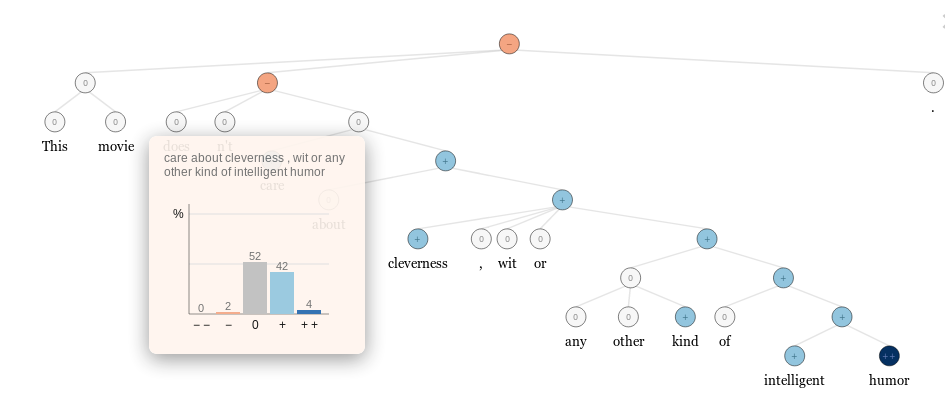
\includegraphics[height=6.5cm]{guide_tree.png}
  \captionof{figure}{Пример результата работы приложения}\label{fig:guide:tree}
\end{center}
